\section{Results}

\subsection{Answers to Question \ref{q1}}

Figures \ref{fig:q1_spatial} and \ref{fig:q1_pgd} show the results of our experiments to determine whether neural networks ``overfit'' to non-robust features during the later stages of training. We distinguish the case of spatial vs. PGD attacks.

\begin{figure}[htb]
    \vspace{-7pt}
    \begin{center}
        \includegraphics[width=0.48\textwidth]{figs/Q1_spatial.eps}
    \end{center}
    \caption{Attack success rates of spatial attacks at various training stages.} \label{fig:q1_spatial}
    \vspace{-10pt}
\end{figure}

\paragraph{For spatial attacks} For spatial attacks (Figure \ref{fig:q1_spatial}), we find that the attack success rate (ASR) fluctuates around a fairly constant rate over the training iterations of the neural network. The ASR for \texttt{rot} remains around 71-80\%, the ASR for \texttt{grid135} remains around 84-90\%, and the ASR for \texttt{grid775} remains around 89-95\%. We conclude that in the case of spatial robustness, neural networks typically do not make a distinction between spatially robust and spatially non-robust features during training, instead using all available features from the very beginning of training.

\begin{figure}[htb]
    \vspace{-7pt}
    \begin{center}
        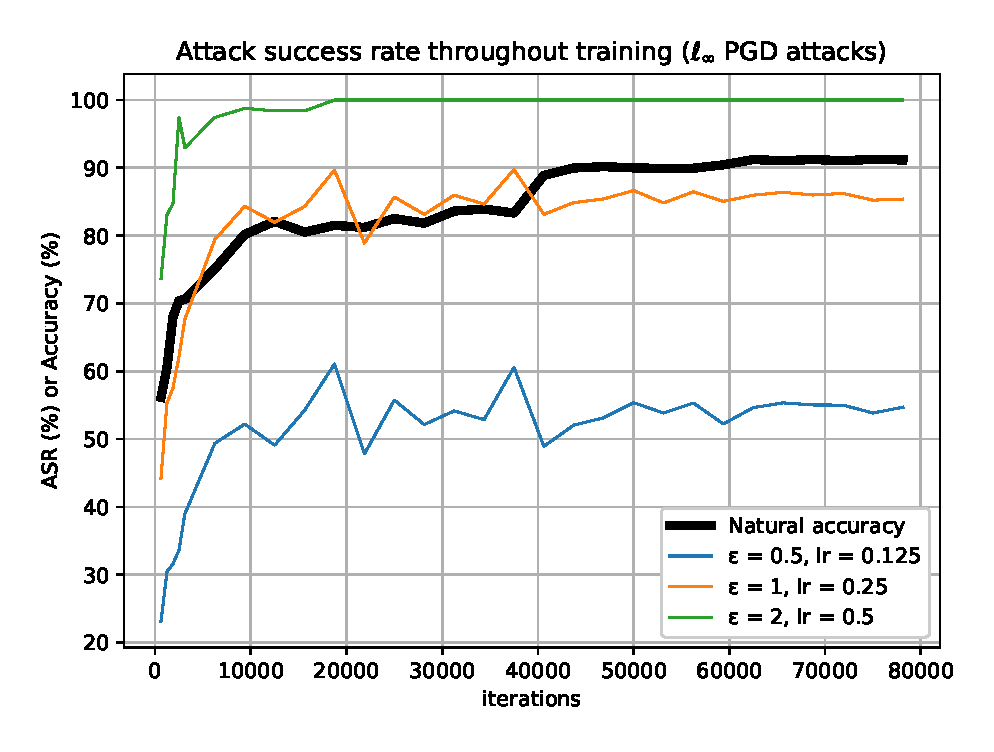
\includegraphics[width=0.48\textwidth]{figs/Q1_PGD.eps}
    \end{center}
    \caption{Attack success rates of \linf PGD attacks at various training stages.} \label{fig:q1_pgd}
    \vspace{-10pt}
\end{figure}

\paragraph{For PGD attacks} Contrary to the case of spatial attacks, we see a slight upward trend in the ASR when performing $L_{\infty}$-norm PGD attacks as training progresses throughout the early stages of training (natural accuracies 60-80\%), as shown in Figure \ref{fig:q1_pgd}. After reaching a natural accuracy of roughly 80\%, ASR fluctuates around a constant level. We can conclude that at a certain stage of training, the neural network will start using non-robust features to increase natural accuracy.

One possible explanation for the difference in results between spatial and PGD attacks is that spatial attacks are a substantially different class of attacks than PGD attacks. In PGD attacks, there is a constraint based on some norm to limit the attack space, whereas in spatial attacks, the attack space is controlled by a maximum degree of rotation and translation.

In both the spatial and the PGD case, it is clear that neural networks do not specifically over-utilize non-robust features during the later stages of training, as ASR remains fairly constant. We can therefore give the following answer to Question \ref{q1}: \textit{increasing natural accuracy causes higher usage of PGD-non-robust features, shown by ASR increasing at the beginning of training. The current goal of optimizing accuracy to its peak level is therefore partially at fault for introducing adversarial vulnerabilities to PGD attacks caused by non-robust features. In the case of spatial robustness, we cannot draw any meaningful conclusion.}

\begin{table*}[t]
\caption{Accuracies achieved from the experiments for Question \ref{q3}. The first row of the table contains natural accuracies, while the remaining rows contain robust accuracies under the attack mentioned in the leftmost column. Each model has four columns of results: ``$D$'' refers to models trained with the natural dataset, while ``$D_R$'' refers to models trained with the robust dataset. The notation $^*$ indicates the model is trained with \texttt{std*} data augmentation. The entries reported in this table are the best ones across the backbone ResNet-18/-34 and learning rates. The raw experiment data is logged in Tables \ref{tab:stnresults} and \ref{tab:spatialattack_g_resnet}.} \label{tab:spatialattack}
    \begin{adjustwidth}{-.5in}{-.5in}  
        \vspace{15pt}
        \begin{center}
            \begin{tabular}{|c|cccc|cccc|cccc|c|}
                \hline
                & \multicolumn{4}{c|}{ResNet-50} & \multicolumn{4}{c|}{G-ResNet} & \multicolumn{4}{c|}{STN} & PTN\footnotemark \\
                Attack & $D$ & $D_R$ & $D^*$ & $D_R^*$ & $D$ & $D_R$ & $D^*$ & $D_R^*$ & $D$ & $D_R$ & $D^*$ & $D_R^*$ & -- \\ 
                \hline
                None &
                94.84 & 84.75 & 93.9 & 83.53 &  % ResNet-50
                \textbf{95.72} & 85.46 & 94.74 & 85.11 &  % G-ResNet
                94.05 & 84.39 & 93.12 & 83.72 &   % STN
                -- \\
                \texttt{rot10} &
                80.97 & 67.78 & 83.24 & 69.67 &  % ResNet-50
                83.56 & 69.22 & \textbf{87.61} & 73.34 &  % G-ResNet
                84.07 & 69.52 & 87.67 & 73.55 &   % STN
                -- \\
                \texttt{rot30} &
                36.77 & 24.94 & 58.75 & 42.62 &  % ResNet-50
                41.74 & 26.95 & 75.38 & 51.97 &  % G-ResNet
                41.01 & 26.4 & \textbf{86.1} & 70.86 &  % STN
                -- \\
                \texttt{grid775,10$^\circ$} &
                63.34 & 52.3 & 67.78 & 55.31 &  % ResNet-50
                68.17 & 55.15 & 75.7 & 60.38 & % G-ResNet
                70.47 & 54.98 & \textbf{77.01} & 60.61 &   % STN
                -- \\
                \texttt{grid135} &
                18.72 & 11.23 & 39.71 & 26.89 &  % ResNet
                21.84 & 11.81 & 56.06 & 36.64 &  % G-ResNet
                22.48 & 11.52 & \textbf{69.47} & 50.76 &   % STN
                -- \\
                \texttt{grid775} &
                15.28 & 9.88 & 35.42 & 24.53 &  % ResNet
                19.36 & 10.78 & 53.19 & 34.57 &  % G-ResNet
                19.94 & 10.09 & \textbf{67.47} & 48.64 &   % STN
                -- \\
                \hline
            \end{tabular}
        \end{center}
    \end{adjustwidth}
    \vspace{-15pt}
\end{table*}

\subsection{Answers to Question \ref{q2}}

The results of our experiments on the dataset $D_{mix}$ are summarized in Figure \ref{fig:mix_results}.  

\begin{figure}[htb]
    \vspace{-7pt}
    \begin{center}
        \begin{minipage}[b]{0.235\textwidth}
            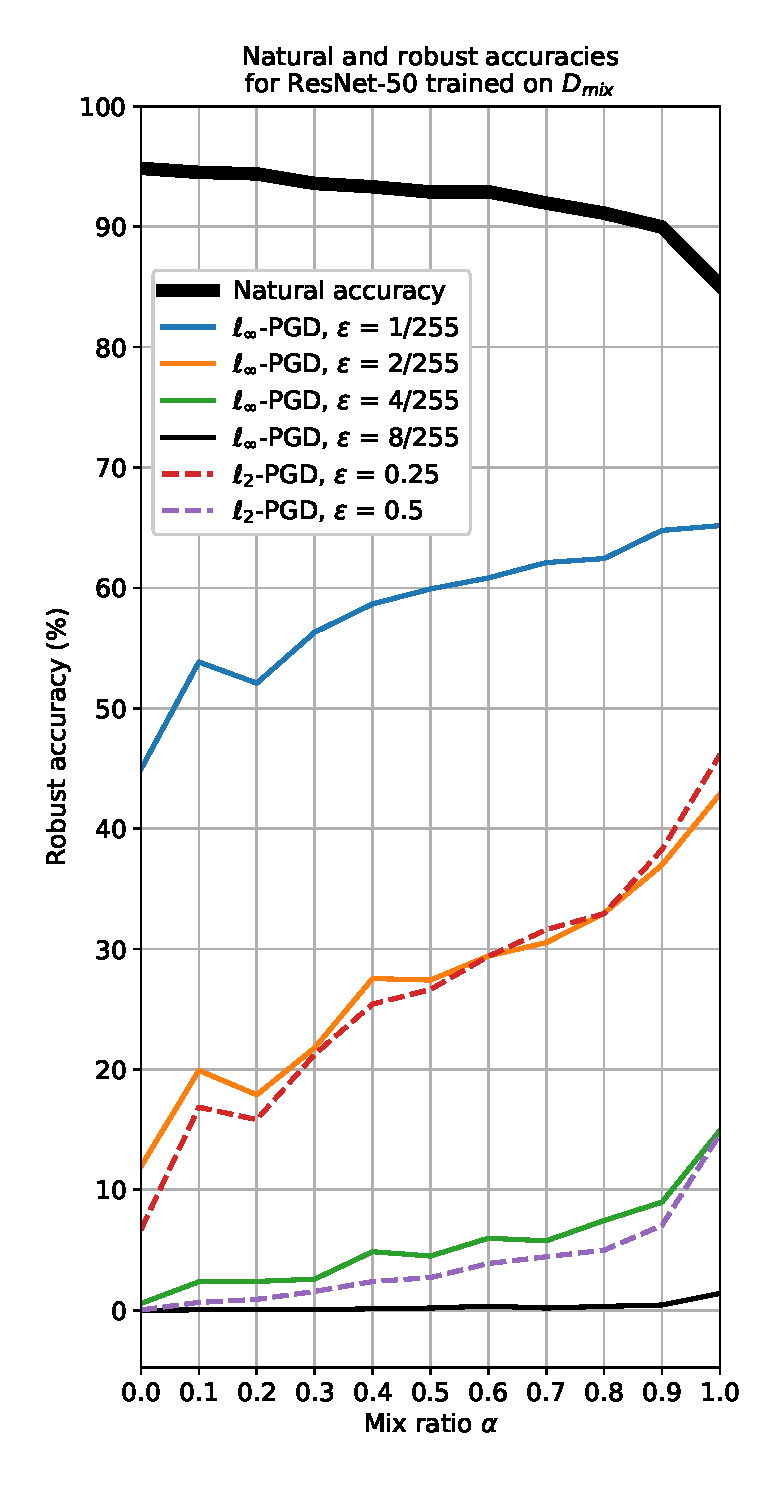
\includegraphics[width=\textwidth]{figs/Q2_resnet.eps}
        \end{minipage}
        \begin{minipage}[b]{0.235\textwidth}
            \includegraphics[width=\textwidth]{figs/Q2_all.eps}
        \end{minipage}
        \vspace{10pt}
        \caption{Left: Robust accuracies of ResNet-50 trained using $D_{mix}$ for different values of the mix ration $\alpha$, where $\alpha=0$ represents using only natural images and $\alpha=1$ represents using only robust images. Right: Comparison accuracies of the robust accuracies of ResNet-50, ResNet-18, and VGG-16 trained on $D_{mix}$ for different values of $\alpha$. For all attacks, we use the learning rates from Section \ref{sec:attacks}.} \label{fig:mix_results}
    \end{center}
    \vspace{-17pt}
\end{figure}

\paragraph{Use of $D_{mix}$ as a defense mechanism} We observe a clear trend that as the mix ration $\alpha$ increases (i.e. the proportion of images from $D_R$ in each training batch increases), the robust accuracy under all considered attacks increases. It is interesting to note that even adding a small amount of images from $D_R$ (e.g. $\alpha=0$ vs. $\alpha=0.1$) greatly increases the robust accuracy, while removing all natural images ($\alpha=0.9$ vs. $\alpha=1$) greatly reduces the natural accuracy. However, even having 10\% of natural images per batch only decreases the natural accuracy by around 4\% compared to using 100\% of natural images. Therefore, using a fixed proportion of images from $D_R$ in each training batch can be considered a fairly effective defense mechanism.

\paragraph{Transferability among different attacks} Ilyas et al. only consider \ltwo-PGD attacks when evaluating their robust dataset $D_R$. Figure \ref{fig:mix_results} (left) shows that $D_R$ is also robust to \linf-PGD attacks (provided the attack is not too strong, as is the case with $\epsilon=\frac{8}{255}$). We conclude that the robustness induced by $D_R$ transfers well among different variations of PGD attack.

\paragraph{Transferability among different architectures} Ilyas et al. generate the robust dataset $D_R$ using a ResNet-50. It is therefore natural to ask whether their generated dataset also has similar robustness-inducing effects on other architectures. Figure \ref{fig:mix_results} (right) shows the results of two different \ltwo-PGD attacks on three different architectures. In all three cases, we observe similar trends to ResNet-50 as $\alpha$ increases. We conclude that a robust dataset generated by one architecture can be used to induce robustness for another architecture.

\subsection{Answers to Question \ref{q3}}
Table \ref{tab:spatialattack} summarizes our results for answering Question \ref{q3}. The models are evaluated under various spatial attack methods. The natural accuracies match baselines in results of \cite{Cohen16, Yang2019}

\paragraph{PGD-robust features do not help boost spatial robustness} Ilyas et al. state that training only with the PGD-robust dataset $D_R$ helps the model to obtain a good degree of robustness in general, but our results clearly demonstrate that this robustness does not apply to the spatial case. In table \ref{tab:spatialattack} we can see that for all architectures, with the same data augmentation procedure, robust accuracy is much lower than its natural counterpart for every spatial attack setting.  

\paragraph{Spatial equivariant networks induce limited spatial robustness with $D_R$} It has been studied in \cite{Yang2019} that several spatial equivariant designs help to boost spatial robustness of the models. However, the results we get from training these specially designed architectures both with $D$ and $D_R$ show that $D_R$ does not further improve the robust accuracy, since all of them do not achieve higher accuracy than when simply trained with $D$.



\footnotetext{For the PTN architecture, due to the training instability for getting the natural accuracy above a meaningful baseline, we omit the results here and leave the results in the appendix.}
